\chapter{Advanced Computer Graphics}
\label{chap:advanced_computer_graphics}

\begin{figure}[ht]
	\hfill
	\begin{minipage}{0.5\textwidth}
		\centering
		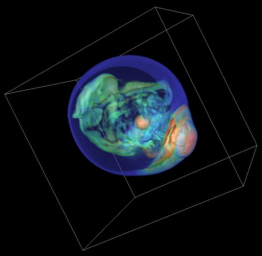
\includegraphics{VTKTextbook-104}\\
		\caption*{\texttt{Volume rendering of a supernova dataset.}}
	\end{minipage}
\end{figure}

\firstletter{C}hapter 3 introduced fundamental concepts of computer graphics.
A major topic in that chapter was how to represent and render geometry using surface primitives such as points, lines, and polygons.
In this chapter our primary focus is on volume graphics.
Compared to surface graphics, volume graphics has a greater expressive range in its ability to render inhomogeneous materials, and is a dominant technique for visualizing 3D image (volume) datasets.

We begin the chapter by describing two techniques that are important to both surface and volume graphics.
These are simulating object transparency using simple blending functions, and using texture maps to add realism without excessive computational cost.
We also describe various problems and challenges inherent to these techniques.
We then follow with a focused discussion on volume graphics, including both object-order and image-order techniques, illumination models, approaches to mixing surface and volume graphics, and methods to improve performance.
Finally, the chapter concludes with an assortment of important techniques for creating more realistic visualizations.
These techniques include stereo viewing, antialiasing, and advanced camera techniques such as motion blur, focal blur, and camera motion.

\section{Transparency and Alpha Values}
\label{sec:transparency_alpha}

Up to this point in the text we have focused on rendering opaque objects — that is, we have assumed that objects reflect, scatter, or absorb light at their surface, and no light is transmitted through to their interior. Although rendering opaque objects is certainly useful, there are many applications that can benefit from the ability to render objects that transmit light. One important
application of transparency is volume rendering, which we will explore in greater detail later in the chapter.

\section{Texture Mapping}

Texture mapping is a technique to add detail to an image without requiring modelling detail. Texture mapping can be thought of as pasting a picture to the surface of an object. The use of texture mapping requires two pieces of information: a \emph{texture map} and \emph{texture coordinates}. The texture map is the picture we paste, and the texture coordinates specify the location where the picture is pasted. More generally, texture mapping is a table lookup for color, intensity, and/or transparency that is applied to an object as it is rendered. Textures maps and coordinates are most often two-dimensional,
but three-dimensional texture maps and coordinates are supported by most new graphics hardware.

\section{Volume Rendering}
\label{sec:volume_rendering}

Until now we have concentrated on the visualization of data through the use of geometric primitives such as points, lines, and polygons.
For many applications such as architectural walk-throughs or terrain visualization, this is obviously the most efficient and effective representation for the data.
In contrast, some applications require us to visualize data that is inherently volumetric (which we refer to as 3D image or volume datasets).
For example, in biomedical imaging we may need to visualize data obtained from an MR or CT scanner, a confocal microscope, or an ultrasound study.
Weather analysis and other simulations also produce large quantities of volumetric data in three or more dimensions that require effective visualization techniques.
As a result of the popularity and usefulness of volume data over the last several decades, a broad class of rendering techniques known as volume rendering has emerged. The purpose of volume rendering is to effectively convey information within volumetric data.

\section{3D Widgets and User Interaction}
\label{sec:3dwui}

Chapter 3 provided an introduction to interaction techniques for graphics (see ``Introducing vtkRenderWindowInteractor'' on page \pageref{pg:rwi} ).
In the context of visualization, interaction is an essential featureof systems that provide methods for data exploration and query. The classes
vtkRenderWindowInteractor and vtkInteractorStyle are core constructs used in VTK to capturewindowing-system specific events in the render window, translate them into VTK events, and then take action as appropriate to that event invocation.
In Chapter 3 we saw how these classes could be used to manipulate the camera and actors to interactively produce a desired view. This functionality, however, is relatively limited in its ability to interact with data. For example, users often wish tointeractively control the positioning of streamline starting points, control the orientation of a clipping plane, or transform an actor. While using interpreted languages (see ``Interpreted Code'' on page \pageref{pg:rwi} ) can go a long way to provide this interaction, in some situations the ability to see what you are doing when placing objects is essential. Therefore, it is apparent that a variety of user interaction techniques is required by the visualization system if it is to successfully support real-world applications.

\section{Bibliographic Notes}

An overview of volume rendering and volume visualization techniques can be found in a tutorial by Kaufman \cite{Kaufman91}. Many of the volume rendering techniques discussed in this chapter are also accessible from research institutions as source code. The shear-warp algorithm is provided within the VolPack rendering library and is available on the Web at \href{http:www-graphics.stanford.edu/software/volpack/}{VolPack} . SUNY Stony Brook offers a turnkey volume visualization system called VolVis to nonprofit and government organizations. Source code and executable versions are available at \href{http://www.cs.sunysb.edu/\~volvis}{VolVis}. In addition, an application called Vis5D is available that applies volume visualization techniques to time varying atmospheric weather data. Vis5D may be obtained from the Web location \href{http://vis5d.sourceforge.net}{Vis5D}. A commercial volume rendering application, VolView, developed on top of The Visualization Toolkit, is available from Kitware for a 30-day trial at \href{http://www.kitware.com/products/volview.html}{VolView}.

\printbibliography


\section{Exercises}

\begin{itemize}

\item In astronomy, photographs can be taken that show the movements of the stars over a period of time by keeping the camera's shutter open. Without accounting for the rotation of the earth, these photographs display a swirl of circular arcs all centered about a common point. Such time lapse photography is essentially capturing motion blur. If we tried to simulate these images using the motion blur technique described in this chapter, they would look different from the photographs. Why is this? How could you change the simple motion blur algorithm to correct this?

\item In **Figure 7-25** we show the difference between stereo rendering with two or one view planes. If you were viewing a rectangle head-on (its surface normal parallel to your direction), what artifacts would be introduced by rendering onto one view plane while using the equations for two planes

\item On some graphics systems transparent objects are rendered using a technique called screen door transparency. Basically, every pixel is either completely opaque or completely transparent. Any value in between is approximated using dithering. So a polygon that was 50 percent opaque would be rendered by drawing only half of the pixels. What visual artifacts does this introduce? What blending problems can arise in using such a technique?

\item In this chapter we describe a few different techniques for anti--aliased rendering. One technique involved rendering a large image and then scaling it down to the desired size using bilinear interpolation. Another technique involved rendering multiple images at the desired size using small camera movements and then accumulating them into a final image. When rendering a model with a surface representation, these two techniques will produce roughly the same result. When rendering a model with a wireframe representation there will be significant differences. Why is this?

\item You need to create a small image of a volume dataset to include on your web page. The dataset contains $512^3$ voxels and the desired image size is$100^2$ pixels. You can use a software object-order method that projects each voxel onto the image, or a software ray casting method that casts one ray for each pixel. Assuming that identical images are created, which method would you select, and why?

\item Two software developers implement volume rendering methods. The first developer uses a software ray casting approach, while the second uses a graphics hardware texture mapping approach. The grayscale images are generated and displayed on a workstation with an 8 bit frame buffer (256 levels of gray). They both use the same interpolation method and the same compositing scheme, yet the two methods produce different images even though the same number of samples from identical locations were used to generate the images. Why is this?

\item In the classification of some medical dataset, scalar values from 100 to 200 represent skin, 200 to 300 represent muscle and 300 to 400 represent bone. The color transfer functions define skin as tan, muscle as red, and bone as white. If we interpolate scalar value and then perform classification, what classification artifacts may appear in the image?

\item The normal encoding example illustrated in **Figure 7-22** produced 82 indices at a recursion depth of two, which would require seven bits of storage. If we instead use a recursion depth of three, how many indices are there? How many unique vector directions does this represent? How many bits of storage does this require?

\item Writing an object-order back-to-front projection algorithm is more difficult for a perspective viewing transformation than a parallel viewing transformation. Explain why this is and draw a 2D diagram of the volume and the viewing frustum that illustrates the issues.

\end{itemize}
